\documentclass[11pt, letterpaper]{report}

%paquetes
\usepackage{tikz}
\usepackage{xcolor}
\usepackage{graphicx}
\usepackage{amsmath}
\usepackage{amssymb}
\usepackage[spanish, activeacute, es-noshorthands]{babel}
\usepackage{colortbl}
\usepackage{float}
\usepackage[utf8]{inputenc}
\usepackage[right = 2.5 cm, left = 2.5 cm, top = 2 cm , bottom = 2 cm]{geometry}
\usepackage{enumitem} %sirve para cambiar el tipo de enumeracion si redefinir comandos ejem: \arabic* \alph*

%configuraciones
\graphicspath{{img/}}
\newcommand{\Center}[1]{
	\begin{center}
		#1
	\end{center}
} %abreviatura para el ambiente center
\newcommand{\Page}[3][c]{
	\begin{minipage}[#1]{#2\textwidth}
		#3
	\end{minipage}
}
\renewcommand{\labelenumi}{$\bullet$} 
\newenvironment{enumTab}{\begin{enumerate}[label=]\item \begin{enumerate}[label=$\bullet$]}{\end{enumerate}\end{enumerate}} %comando para realizar enumeraciones con cierto margen
\newenvironment{block}[1]{\hspace{-0.8 cm}\textbf{\Large #1}}{\vspace{3 mm}} %ambiente importante que define una parte del reporte.
\newenvironment{question}[2]{\hspace{-0.8 cm}\textbf{#1) #2\\\\}}{\vspace{3 mm}} % define una pregunta, recibe como primer parametro al número y siguiente es la pregunta
\newcommand{\bib}[2]{ \textbf{\large #1:} \small #2\\} %forma sencilla de crear una referencia, como primer parametro recibe el titulo y el segundo el lugar a consultar
\newcommand{\note}[1]{\small \textbf{Nota:} #1} %comando que inserta una nota al texto
\spanishdecimal{.}
%comandos personales
%este commando sirve para crear bolas con enumeración
\newcommand*{\enumBall}[1]
		{
		\footnotesize\protect\tikz[baseline=-3pt]
		\protect\node[scale=.7, circle, ball color = white]{\color{black}\Large\bf #1};
		}
	
	
%%%%%%%%%%%%%%%%%%%%%%%%%%%%%%%%%%%%%%%%%%%%%%%%%%%%%%%%%%%%%%%%%%%%%%%%%%
%%%%%%%%%%%%%%%%%%%%%%% DOCUMENT BODY %%%%%%%%%%%%%%%%%%%%%%%%%%%%%%%%%%%%
%%%%%%%%%%%%%%%%%%%%%%%%%%%%%%%%%%%%%%%%%%%%%%%%%%%%%%%%%%%%%%%%%%%%%%%%%%	

\begin{document} 
	
	%%%%%%%%%%%%%%%%%%%%%%%%%%%%%%%%%%%%%
	%%%%%%%%%%%%% HEADER %%%%%%%%%%%%%%%%
	%%%%%%%%%%%%%%%%%%%%%%%%%%%%%%%%%%%%%
	%%%% BLOQUE DE DATOS %%%
\newcommand{\Title}{
	Práctica de Laboratorio \#3
	Multiplexores
} %Titulo del reporte

\newcommand{\LogoUniversity}{img/logo.jpg} %localizacion del logo
\newcommand{\NameUniversity}{Universidad Galileo} %Nombre de la universidad
\newcommand{\Date}{
	Guatemala, 6 de marzo de 2020
} %Fecha de entrega
\newcommand{\Faculty}{Facultad FISICC} %Nombre de la facultad
\newcommand{\Course}{
	Curso: Sistemas de Arquitectura
} %Nombre del curso
\newcommand{\ID}{
	Carnet: 1800 2955
}
\newcommand{\Student}{
	Alumno: Josu\'e Benyamin Isa\'i Galeano Morales
} %Nombre del estudiante
\newcommand{\Section}{
	Secci\'on: A
} %Sección del estudiante
\newcommand{\Schedule}{
	Horario de laboratorio: 18:00 a 19:00
} %Horario
\newcommand{\Assistant}{
	Auxiliar: Evelyn Cruz
} %Persona encargada
\newcommand{\Day}{
	Día de laboratorio: viernes
} %Dia en que recibe
%% FIN BLOQUE DE DATOS%%


%% NO ES NECESARIO MODIFICAR ESTA PARTE %%
\textbf{
	\small
	\hspace{-1 cm}
	\begin{minipage}{0.15\textwidth}
		%%%%%%%%%%%%%%%%% LOGO %%%%%%%%%%%%%%%%%%%%%%%%%%%%%%%
		\includegraphics[scale=0.5]{\LogoUniversity}
	\end{minipage}
	\begin{minipage}{0.7\textwidth}
		\resizebox{1.25\textwidth}{!}{
			\begin{tabular}{ll}
				\hline 
				%%%%% PARTE SUPERIOR DE LA TABLA DE DATOS %%%%%%%%%%%%%%%%%%%%%%%
				\NameUniversity & \Date \\
				\hline
				\rowcolor{lightgray}
				\Faculty & \Student\\
				\hline 
				\Course & \ID\\
				\hline\rowcolor{lightgray}
				\Section & \Schedule\\
				\hline 
				\Assistant & \Day\\
				\hline
			\end{tabular}
		}
	\end{minipage}
}

\vspace{0.5cm}
\begin{tikzpicture}
\hspace{-1 cm}
\draw (0.1,0.1) rectangle (1.043\textwidth,0.9);
\draw[line width=0.7mm] (0,0) rectangle (1.05\textwidth,1);
\node[font=\Large] at (0.525\textwidth, 0.45) {\textbf{\Title}};
\end{tikzpicture}		

\vspace*{0.5 cm}
 %incluimos la parte del header en el documento, note que header es como escribir dentro de un ambiente document por lo tanto no debe llevar definición de clase ni definiciones que se hagan exclusivamente en el preambulo.
	
	%%%%%%%%%%%%%%%%%%%%%%%%%%%%%%%%%%%%%
	%%%%%%%%%%%% OBJETIVOS %%%%%%%%%%%%%%
	%%%%%%%%%%%%%%%%%%%%%%%%%%%%%%%%%%%%%
	\begin{block}{Objetivos:}
		\begin{enumTab}
			\item Entender el funcionamiento de los diodos emisores de luz en corriente directa.
		\end{enumTab}
	\end{block}

	%%%%%%%%%%%%%%%%%%%%%%%%%%%%%%%%%%%%%
	%%%%%%%%%%%%% RESUMEN %%%%%%%%%%%%%%%
	%%%%%%%%%%%%%%%%%%%%%%%%%%%%%%%%%%%%%		
	\begin{block}{Resumen:}
		
		En la pr'actica se conectaron 4 LEDs de diferentes colores para ver el funcionamiento que estos presentaban cuando eran sometidos a una diferencia de potencial de 5V y la configuraci\'on serie prove\'ida en la pr\'actica.
	\end{block}
		
	%%%%%%%%%%%%%%%%%%%%%%%%%%%%%%%%%%%%%
	%%%%%%%%%%%%% TEORIA %%%%%%%%%%%%%%%%
	%%%%%%%%%%%%%%%%%%%%%%%%%%%%%%%%%%%%%
	\begin{block}{Teor'ia:}
	
		\textbf{Los circuitos Serie} son una configuraci'on especial de componentes en un circuito, la caracter'istica de estos circuitos es que la corriente que fluye por todos sus miembros es la misma, por lo mismo la resistencia equivalente de resistores en serie es la suma de sus valores debido a que todos ellos se oponen a la misma corriente.
	  
		\begin{figure}[H]
		\hfill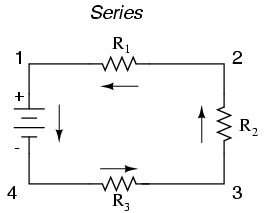
\includegraphics[scale=0.5]{serie.png}\hspace*{\fill}
		\caption{\textbf{\emph{Circuito Serie}}}
		\end{figure}
		
		\textbf{\emph{LED}} es un diodo semiconductor que por sur propiedades de construcci\'on es capaz de emitir luz como sus siglas los dicen, se trata de un diodo de uni\'on tipo p-n en el cual cuando la corriente fluye a trav\'es del mismo este se activa y es capaz de emitir luz, un dato importante que cabe resaltar de un LED es que el color varia según el ancho de la conocida banda prohibida.
		
		\begin{minipage}{.5\textwidth}
			\begin{figure}[H]
				\Center{
					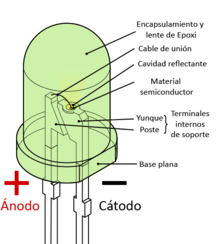
\includegraphics[scale=.4]{LED.png}
					\caption{\textbf{LED}}
				}
			\end{figure}
		\end{minipage} 
		\begin{minipage}{.5\textwidth}
			\begin{figure}[H]
				\Center{
					
\includegraphics[scale=.8]{Led_esquematico.png}
					\caption{\textbf{diagrama esquematico LED}}
				}
			\end{figure}
		\end{minipage}
	\end{block}
		
	%%%%%%%%%%%%%%%%%%%%%%%%%%%%%%%%%%%%%
	%%%%%%%%%% DATOS PRACTICOS %%%%%%%%%%
	%%%%%%%%%%%%%%%%%%%%%%%%%%%%%%%%%%%%%
	\begin{block}{Datos Pr'acticos:}
		
		\vspace*{.5cm}
		\Page{.5}{
			\begin{figure}[H]
				\Center{
					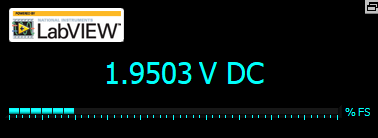
\includegraphics[scale=.5]{vamarillo.png}
					\caption{\textbf{voltaje LED amarillo}}
				}
			\end{figure}
		}
		\Page{.5}{
			\begin{figure}[H]
				\Center{
					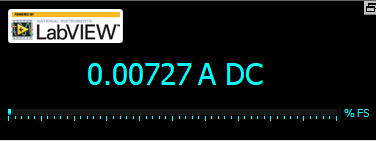
\includegraphics[scale=.5]{iamarillo.png}
					\caption{\textbf{corriente LED amarillo}}
				}
			\end{figure}
		}
	
		\Page{.5}{
			\begin{figure}[H]
				\Center{
					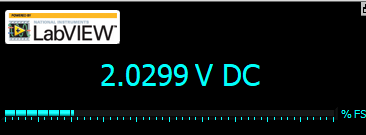
\includegraphics[scale=.5]{vverde.png}
					\caption{\textbf{voltaje LED verde}}
				}
			\end{figure}
		}
		\Page{.5}{
			\begin{figure}[H]
				\Center{
					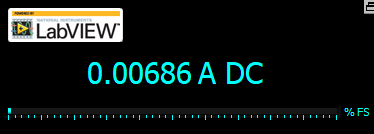
\includegraphics[scale=.5]{iverde.png}
					\caption{\textbf{corriente LED verde}}
				}
			\end{figure}
		}
	
		\Page{.5}{
			\begin{figure}[H]
				\Center{
					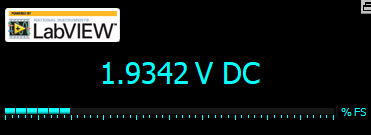
\includegraphics[scale=.5]{vrojo.png}
					\caption{\textbf{voltaje LED rojo}}
				}
			\end{figure}
		}
		\Page{.5}{
			\begin{figure}[H]
				\Center{
					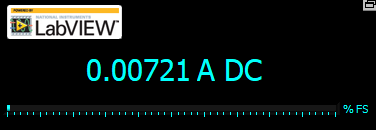
\includegraphics[scale=.5]{irojo.png}
					\caption{\textbf{corriente LED rojo}}
				}
			\end{figure}
		}
	
		\Page{.5}{
			\begin{figure}[H]
				\Center{
					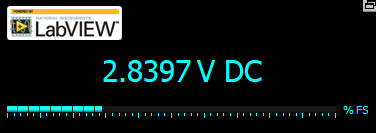
\includegraphics[scale=.5]{vazul.png}
					\caption{\textbf{voltaje LED azul}}
				}
			\end{figure}
		}
		\Page{.5}{
			\begin{figure}[H]
				\Center{
					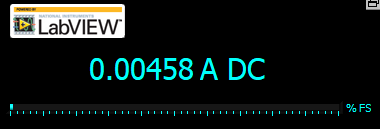
\includegraphics[scale=.5]{iazul.png}
					\caption{\textbf{corriente LED azul}}
				}
			\end{figure}
		}
	
	\vspace*{0.6cm}
	\Center{
		\LARGE
		\begin{tabular}{|ccc|}
			\hline
			\rowcolor{yellow}
			\textbf{Color}&\textbf{Voltaje}&\textbf{Corriente}\\
			\hline
			\hline
			Amarillo&1.95V&7.27mA\\\hline
			Verde&2.03V&6.86mA\\\hline
			Rojo&1.93V&7.21mA\\\hline
			Azul&2.84V&4.58mA\\\hline
		\end{tabular}
	}
	
	\end{block}
	
	%%%%%%%%%%%%%%%%%%%%%%%%%%%%%%%%%%%%%
	%%%%%%%%% CALCULOS TEORICOS %%%%%%%%%
	%%%%%%%%%%%%%%%%%%%%%%%%%%%%%%%%%%%%%
	\begin{block}{C\'alculos Te\'oricos:\\}
		
		\textbf{Para Corriente}\\
		\Page{.33}{$V_1-V_R-V_D=0$}
		\Page{.33}{$5v-I(V)390\Omega-V=0$}
		\Page{.33}{$$I(V)=\frac{5v-V}{390\Omega}$$}
		
		\textbf{C\'alculos Te\'oricos}\\
		\Page{.33}{$I(3v)=5.12mA$ (LED azul)}
		\Page{.33}{$I(1.8v)=8.21mA$ (LED rojo)}
		\Page{.35}{$I(2.1v)=7.44mA$ (LED amarillo)}
		\Page{.33}{$I(2.2v)=7.44mA$ (LED verde)}
		
		\textbf{C\'alculos de Pr\'actica}\\
		\Page{.33}{$I(2.84v)=5.54mA$ (LED azul)}
		\Page{.33}{$I(1.93v)=7.87mA$ (LED rojo)}
		\Page{.38}{$I(1.95v)=7.82mA$ (LED amarillo)}
		\Page{.33}{$I(2.03v)=7.62mA$ (LED verde)}
		
		\vspace{.5cm}
		\Large
		\Center{
			\begin{tabular}{|c|c|}
				\hline
				\rowcolor{yellow}
				\multicolumn{2}{|c|}{Error Porcentual}\\
				\hline
				\rowcolor{yellow}
				Color&Error\\
				\hline
				\hline
				Amarillo&5.11\%\\
				\hline
				Verde&7.19\%\\
				\hline
				azul&8.2\%\\
				\hline
				rojo&4.14\%\\
				\hline
			\end{tabular}
		}
		
		
	\end{block}
			
	%%%%%%%%%%%%%%%%%%%%%%%%%%%%%%%%%%%%%
	%%%%%%%%%%% CONCLUSIONES %%%%%%%%%%%%
	%%%%%%%%%%%%%%%%%%%%%%%%%%%%%%%%%%%%%
	\vspace{3 mm}
	\begin{block}{Conclusiones:}
	\begin{enumTab}
		\item Los LEDs por sus propiedades de construcci\'on son capaces de emitir luz al ambiente.
		\item Es necesario colocar una resistencia en serie al LED, ya que estos diodos tienen una baja resistencia, entonces el diodo se quemar\'ia sino la tuviera.
		\item La separaci\'on entre las bandas es la que influye en el color que emite el diodo ya que esta ligada a la longitud de onda de la misma.
	\end{enumTab}
	\end{block}
		
		
	%%%%%%%%%%%%%%%%%%%%%%%%%%%%%%%%%%%%%
	%%%%%%%%%%% BIBLIOGRAFIA %%%%%%%%%%%%
	%%%%%%%%%%%%%%%%%%%%%%%%%%%%%%%%%%%%%
	\begin{block}{Bibliograf'ia:}
	
		\bib{Circuito Serie - Wikipedia}{https://es.wikipedia.org/wiki/Circuito\_en\_serie}
		\hspace*{.5cm}\bib{LED - Wikipedia}{https://es.wikipedia.org/wiki/Led}
	\end{block}
		
\end{document}
